\documentclass[hidelinks,aspectratio=169]{beamer}
\usepackage[italian]{babel} 
\usepackage[utf8]{inputenc} 
\usepackage{fourier} 

%Slide colors
\usetheme{Madrid}
%\usecolortheme{beaver}

% Images
\usepackage{graphicx}
\usepackage{caption}
\usepackage{subcaption}
\usepackage{float}
\graphicspath{{Images}}

% Stop hyphenation
\usepackage[none]{hyphenat}

% Minipages in the same line
\usepackage{tabularx}

% Coloring links
\usepackage{xcolor}

% Enumerate abc
\usepackage{enumerate}

% Redefines caption setup in way to remove "Figure:"
\usepackage{caption}
\captionsetup[figure]{labelformat=empty}

% License
\usepackage[
type={CC},
modifier={by-nc-sa},
version={4.0},
]{doclicense}

%------------------- Commands zone --------------------

%Command to zoom in
\usepackage{mwe}
\makeatletter
\newsavebox\zb@x
\newcounter{z@@m}
\usepackage{calc}
\newdimen\B@r\newdimen\P@r
\newdimen\@zw\newdimen\@zh\newdimen\@zd

\newcommand{\zoombox}[2][0]{%
	\leavevmode%
	\sbox\zb@x{#2}%
	\setlength\B@r{1pt*\ratio{\wd\zb@x}{\ht\zb@x+\dp\zb@x}}%
	\setlength\P@r{1pt*\ratio{\paperwidth}{\paperheight}}%
	\ifdim\B@r>\P@r\relax%
	\setlength\@zw{\wd\zb@x}\setlength\@zh{\@zw*\ratio{\paperheight}{\paperwidth}}%
	\setlength\@zd{(\@zh-\ht\zb@x-\dp\zb@x)*\real{0.5}+\dp\zb@x}%
	\setlength\@zh{\@zh-\@zd}%
	\else%
	\setlength\@zh{\ht\zb@x+\dp\zb@x}%
	\setlength\@zw{\@zh*\ratio{\paperwidth}{\paperheight}}%
	\setlength\@zh{\ht\zb@x}\setlength\@zd{\dp\zb@x}%
	\fi%
	\makebox[0pt][l]{\makebox[\wd\zb@x][c]{\makebox[\@zw][l]{%
				\pdfdest name {zbfs\thez@@m} fitr
				width  \@zw\space
				height \@zh\space
				depth  \@zd\space
	}}}%
	\pdfdest name {zb\thez@@m} fitr
	width  \wd\zb@x\space
	height \ht\zb@x\space
	depth  \dp\zb@x\space
	\immediate\pdfannot 
	width  \wd\zb@x\space
	height \ht\zb@x\space
	depth  \dp\zb@x\space
	{%
		/Subtype/Link/H/N
		/Border [0 0 #1 [1 2]]
		/A <<
		/S/JavaScript
		/JS (
		if(typeof(zoomed)=='undefined'||!zoomed){
			var lastView=this.viewState;
			if(app.fs.isFullScreen) this.gotoNamedDest('zbfs\thez@@m');
			else this.gotoNamedDest('zb\thez@@m');
			zoomed=true;
		}else{
			this.viewState=lastView;
			zoomed=false;
		}
		)
		>>
	}%
	\usebox{\zb@x}%
	\stepcounter{z@@m}%
} 
\makeatother

%------------------- Header --------------------
\title[Creazione di una piattaforma web]{\textbf{Creazione di una piattaforma web per l'esercitazione del nuovo esame della patente nautica secondo l'emendamento "DD 131 del 31 maggio 2022}}
\author{Francesco Rombaldoni}
\date{8 Febbraio 2022/2023}

\begin{document}
	
	\begin{frame}
		\maketitle
		
		\vspace*{\fill}
		\centering
		\fboxrule=2pt
		\fbox
		{
			\begin{minipage}{0.9\linewidth}
				\small{Il seguente documento è ottimizzato per la visualizzazione digitale con \href{https://get.adobe.com/it/reader/}{\textcolor{blue}{Adobe~Acrobat~Reader}}.}  
			\end{minipage}
		}
	\end{frame}
	
	\begin{frame}
		\tableofcontents
	\end{frame}
	
	\section{Selezione di un "single-board" pc}
	\begin{frame}{Selezione di un "single-board" pc}
		\begin{itemize}
			\item Durante la fase preliminare del progetto è stata data molta importanza alla selezione di un "single-board" pc adeguato per fare da server per il sito internet. Dato che il dispositivo sarebbe dovuto rimanere acceso interrottamente per molto tempo, fondamentale è stata la valutazione dei costi/benefici, ovvero la quantità di energia assorbita rispetto alle prestazioni erogate. 
		\end{itemize}
		\vspace*{2mm}
		\begin{center}
			\zoombox{
\includegraphics[scale=0.2]{RISC-vs-CISC-chips.png}}
		\end{center}
	\end{frame}
	
	\begin{frame}{Selezione di un "single-board" pc}
		\vspace*{-3mm}
		\begin{center}
			{\Large \textbf{RISC}}
		\end{center}
		\vspace*{3mm}
		\begin{tabularx}{\linewidth}{XXXX}
			{
				\begin{minipage}{\linewidth}
					\centering
					\zoombox{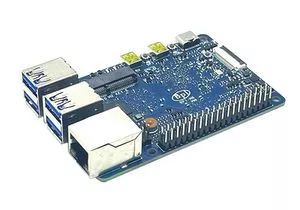
\includegraphics[scale=0.22]{Risc/1Banana_Pi.png}}
					\captionof{figure}{BPI-M6.}
					\zoombox{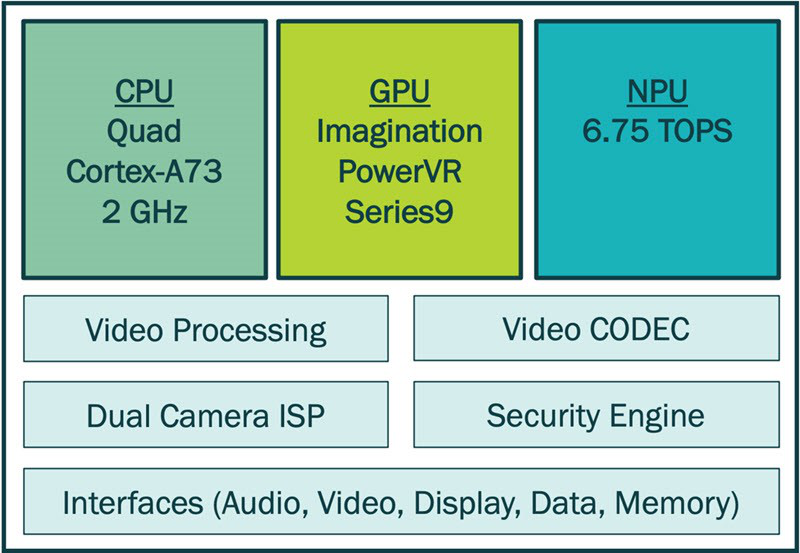
\includegraphics[scale=0.2]{Risc/1synaptics-vs680-block-diagram.png}}
					\captionof{figure}{Synaptics-vs680.}
				\end{minipage}
			}&{
				\begin{minipage}{\linewidth}
					\centering
					\zoombox{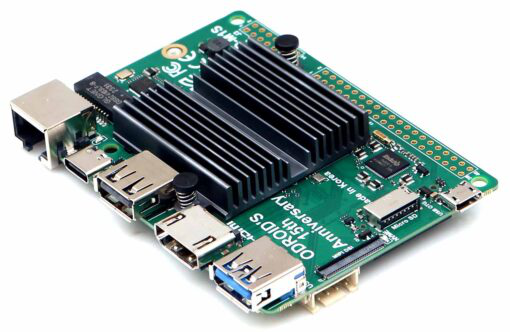
\includegraphics[scale=0.13]{Risc/2Odroid.png}}
					\captionof{figure}{Odroid-M1S.}
					\zoombox{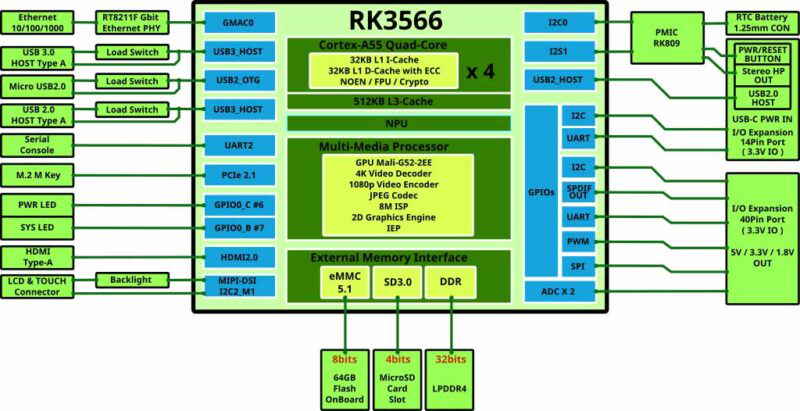
\includegraphics[scale=0.2]{Risc/2m1s_rk3566.png}}
					\captionof{figure}{Rk3566.}
				\end{minipage}
			}&{
			\begin{minipage}{\linewidth}
				\centering
				\zoombox{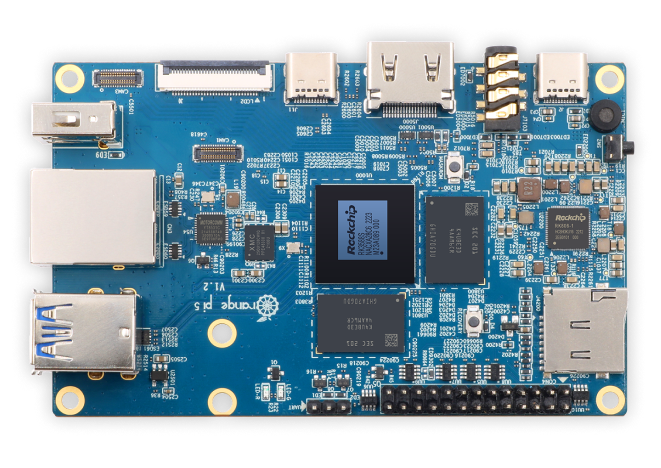
\includegraphics[scale=0.085]{Risc/3orange-pi-5.png}}
				\captionof{figure}{OPI-5.}
				\zoombox{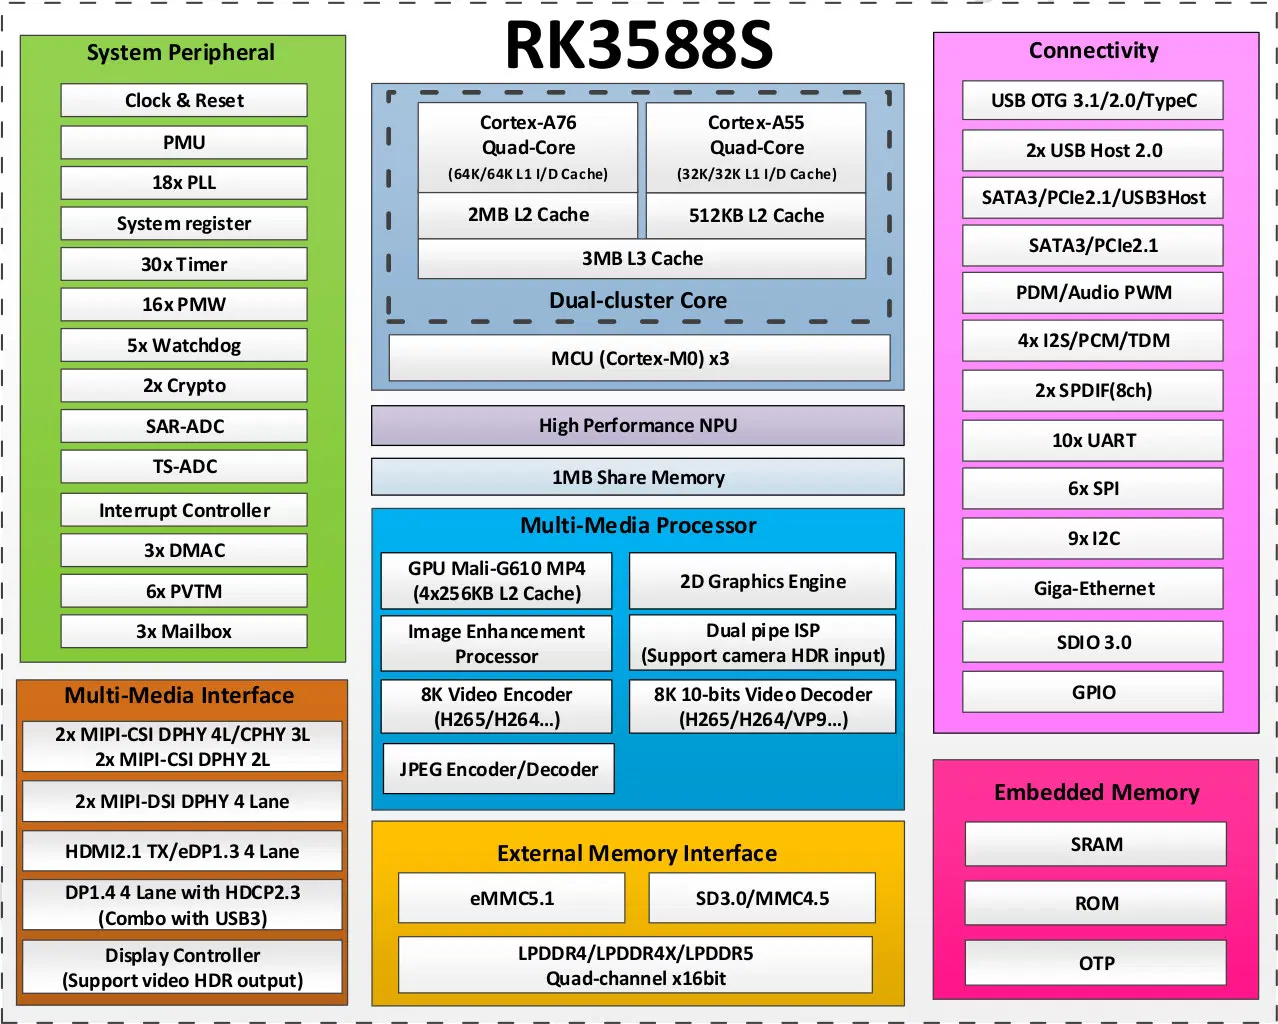
\includegraphics[scale=0.05]{Risc/3RK3588S.png}}
				\captionof{figure}{Rk3588S.}
			\end{minipage}
		}&{
			\begin{minipage}{\linewidth}
				\centering
				\zoombox{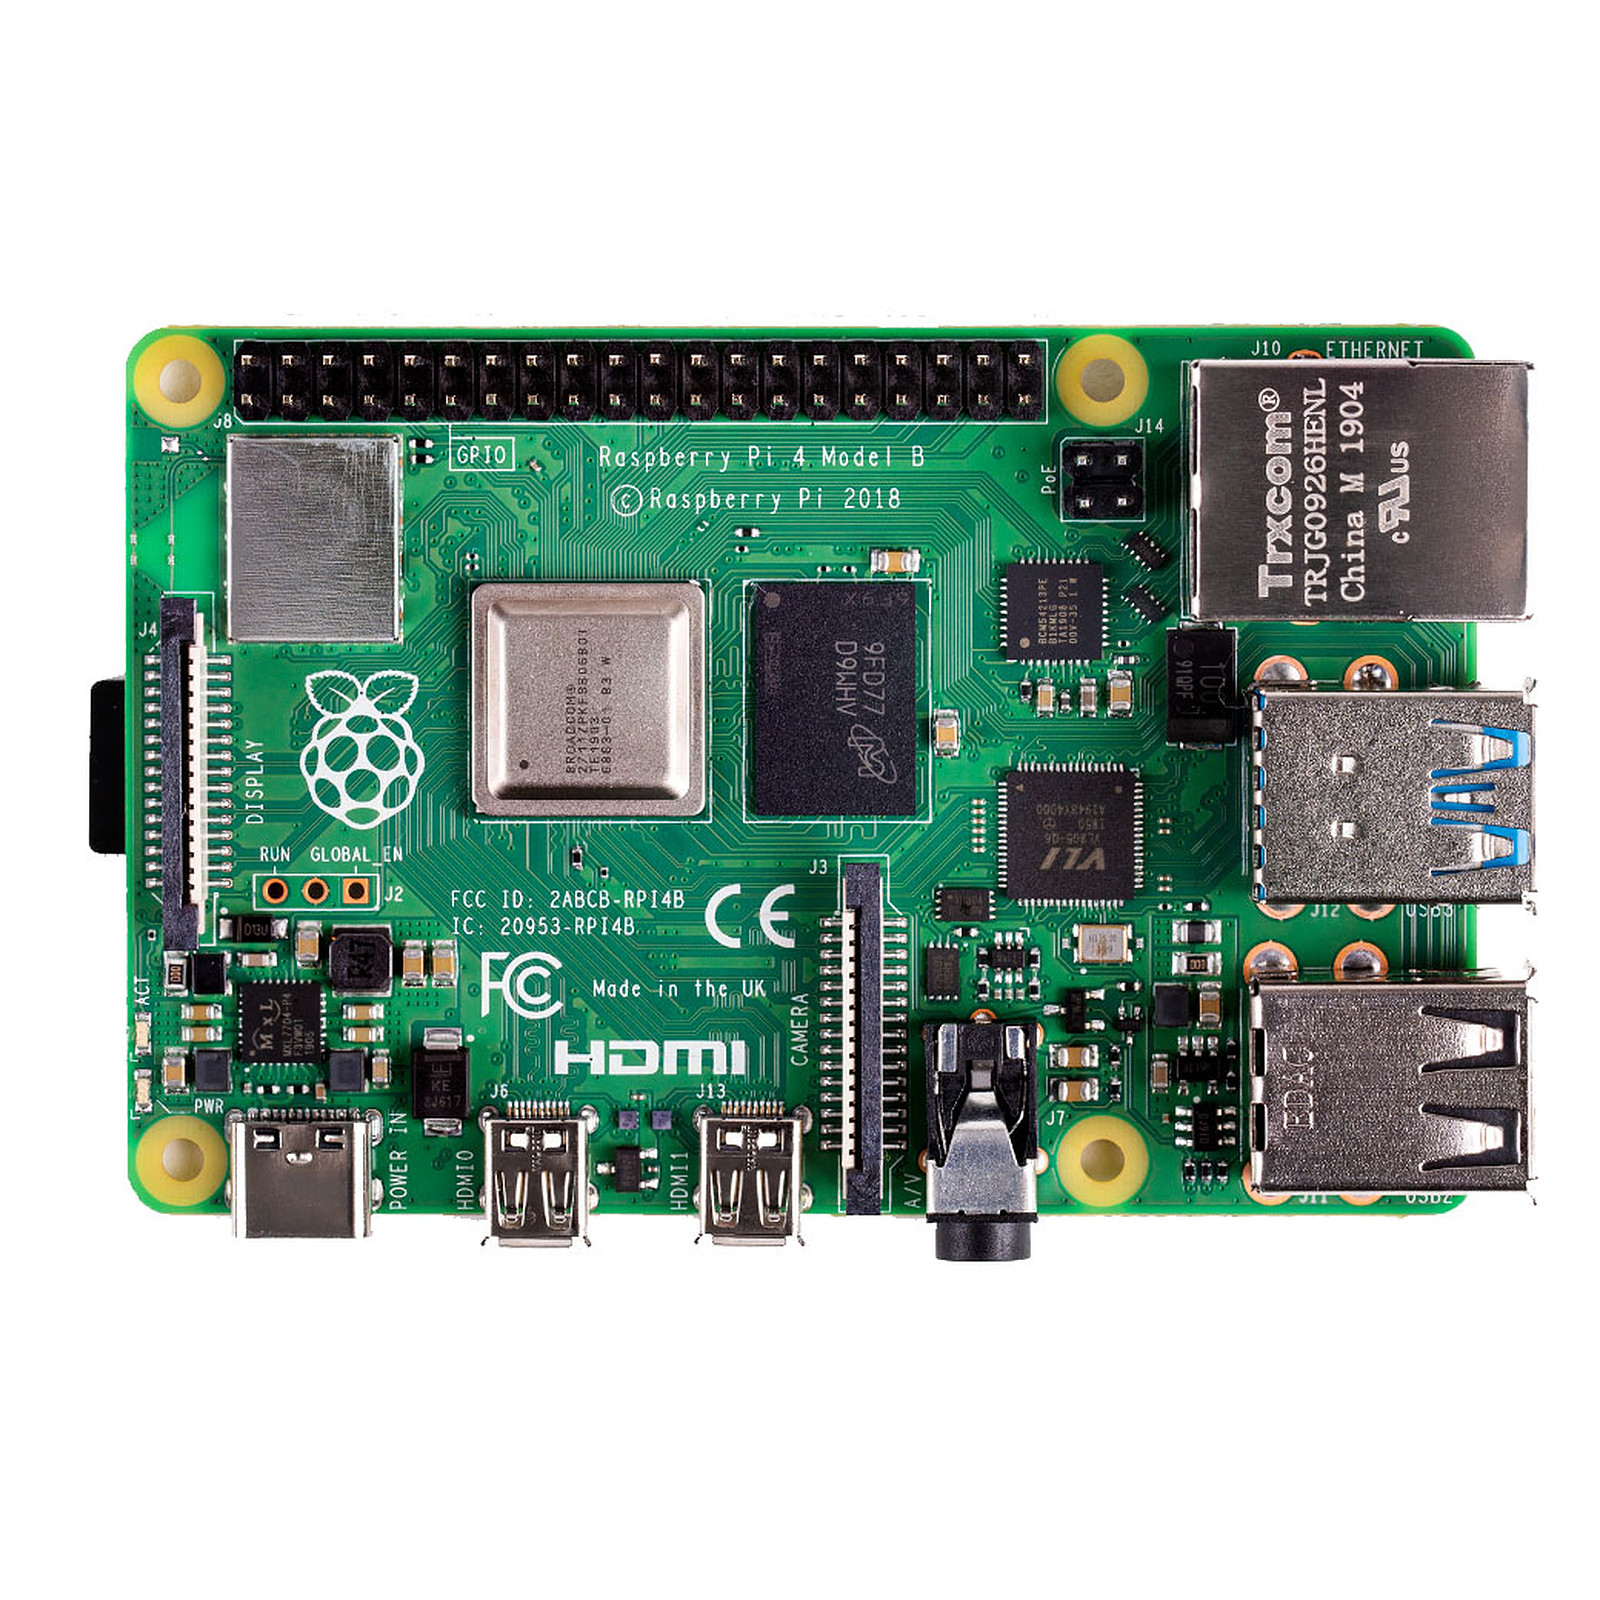
\includegraphics[scale=0.17]{Risc/4Raspberry_pi_4}}
				\captionof{figure}{RPI-4.}
				\zoombox{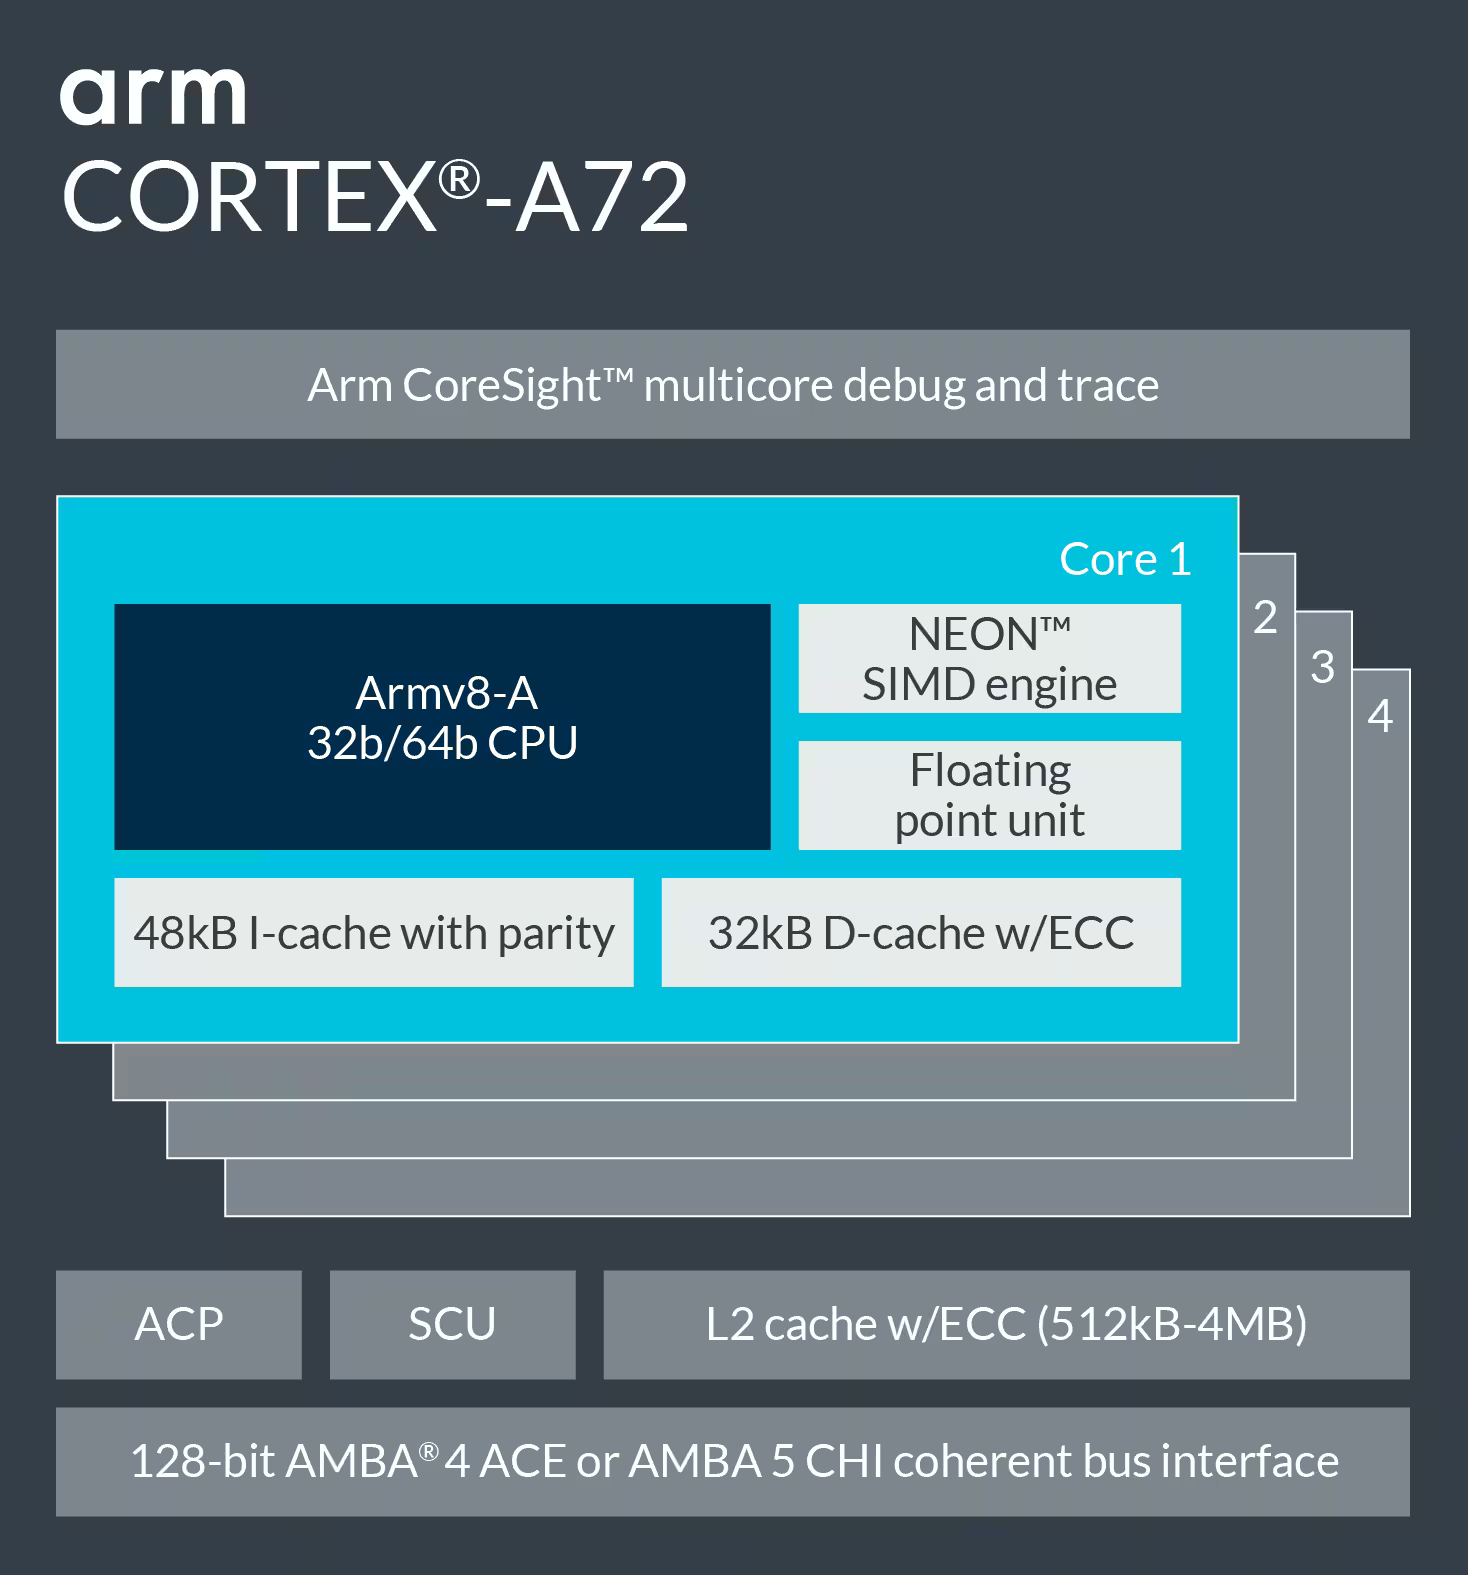
\includegraphics[scale=0.03]{Risc/4Cortex-A72}}
				\captionof{figure}{Cortex-A72.}
			\end{minipage}
			}
		\end{tabularx}
	\end{frame}
	
	\begin{frame}{Selezione di un "single-board" pc}
		\begin{center}
			{\Large \textbf{CISC}}
		\end{center}
		\begin{tabularx}{\linewidth}{XX}
			{
				\begin{minipage}{\linewidth}
					\centering
					\zoombox{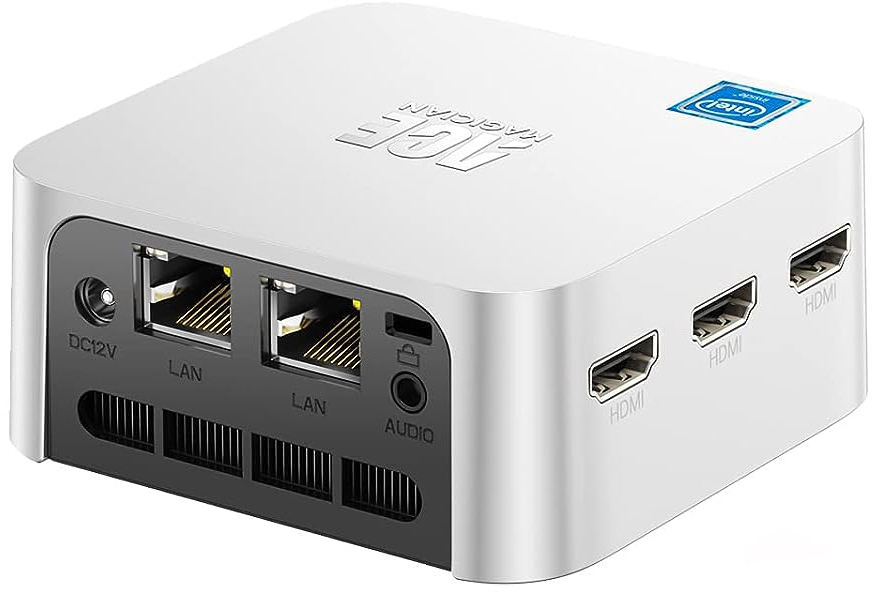
\includegraphics[scale=0.3]{Cisc/1ACEMAGICIAN-T8Plus.png}}
					\captionof{figure}{Acemagician-T8Plus.}
					\zoombox{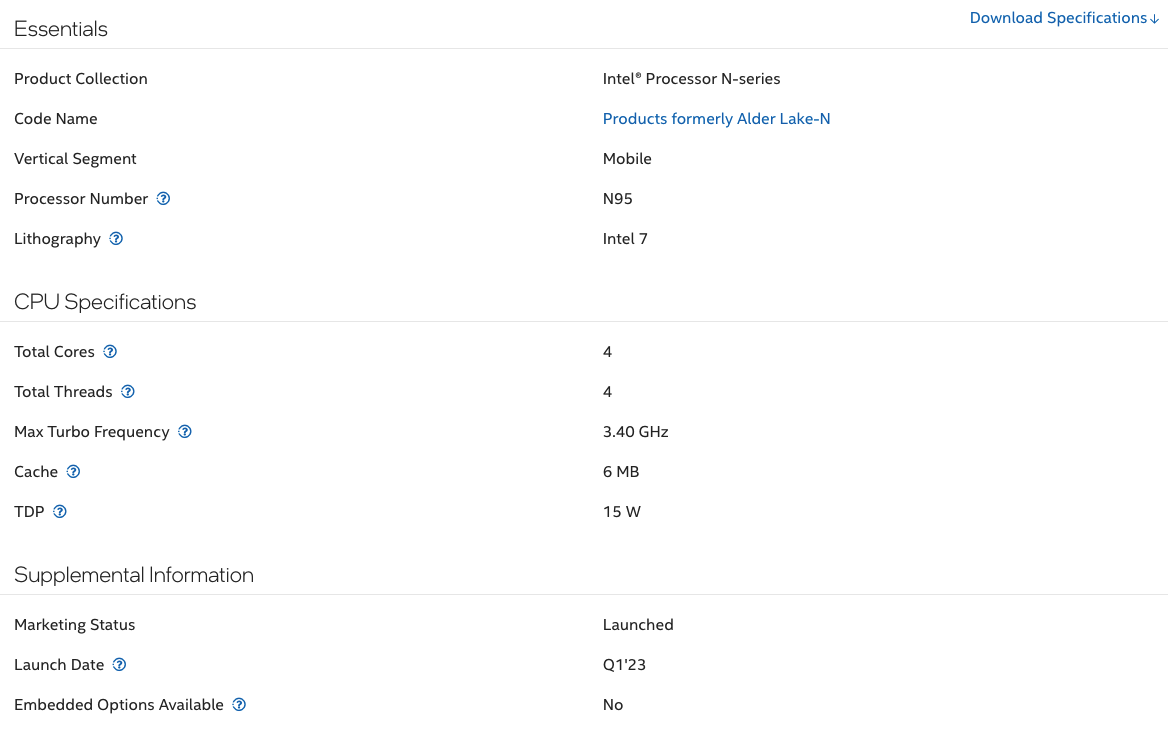
\includegraphics[scale=0.12]{Cisc/1Intel Alder Lake-N95.png}}
					\captionof{figure}{Intel Alder Lake-N95.}
				\end{minipage}
			}&{
				\begin{minipage}{\linewidth}
					\centering
					\zoombox{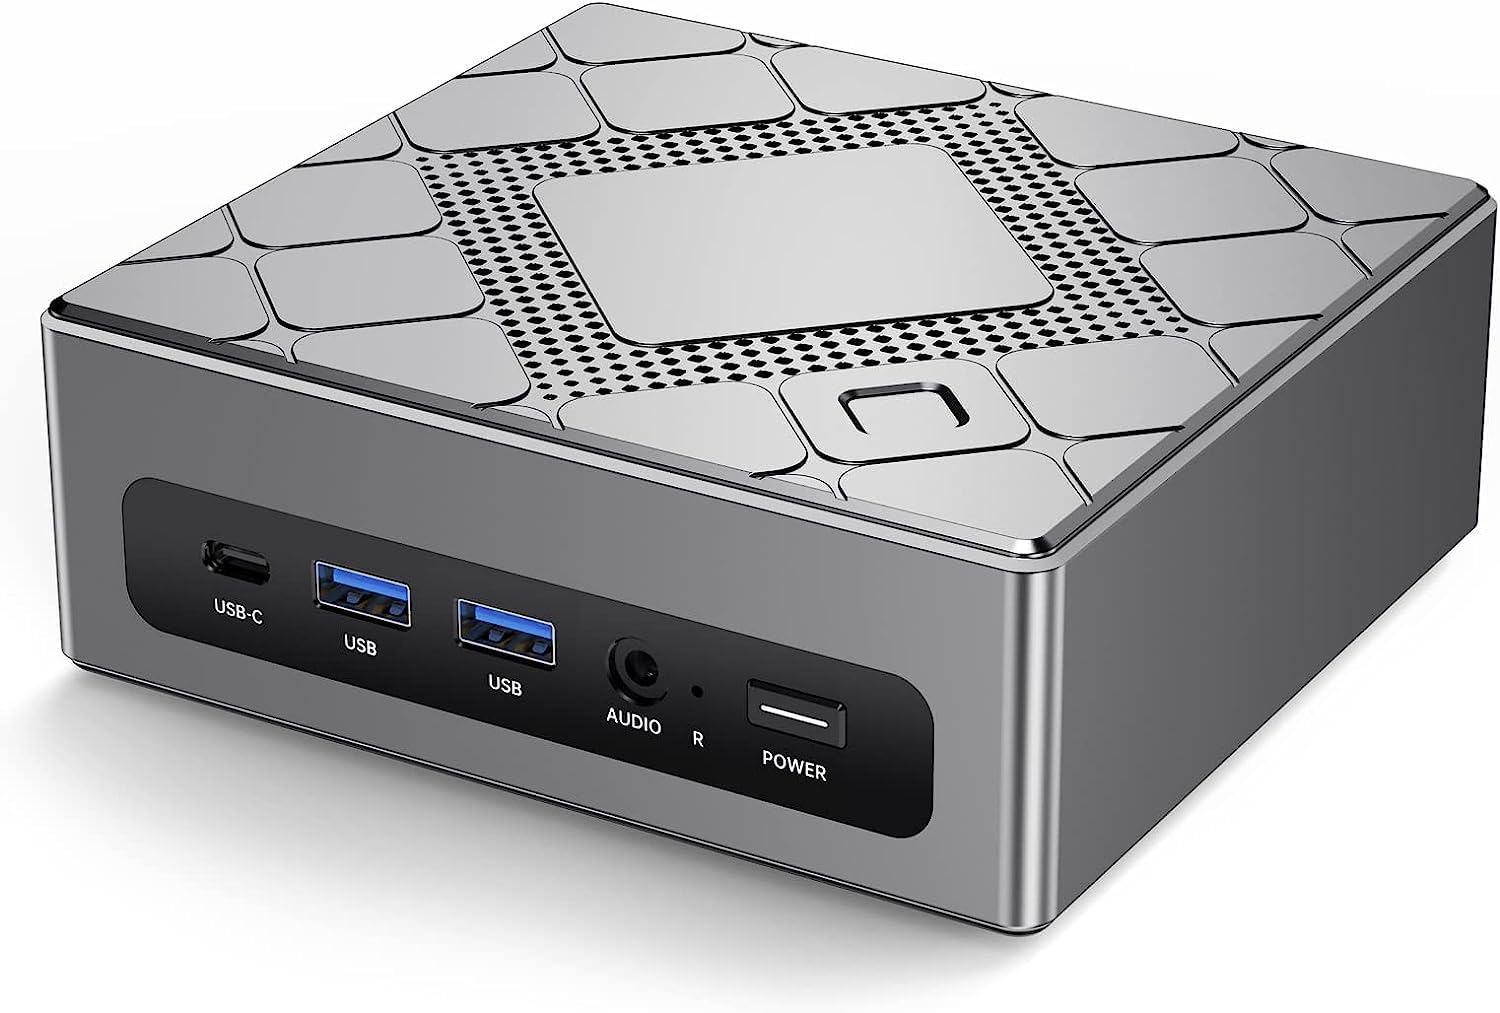
\includegraphics[scale=0.18]{Cisc/2ACEMAGICIAN-CK10.png}}
					\captionof{figure}{Acemagician-CK10.}
					\zoombox{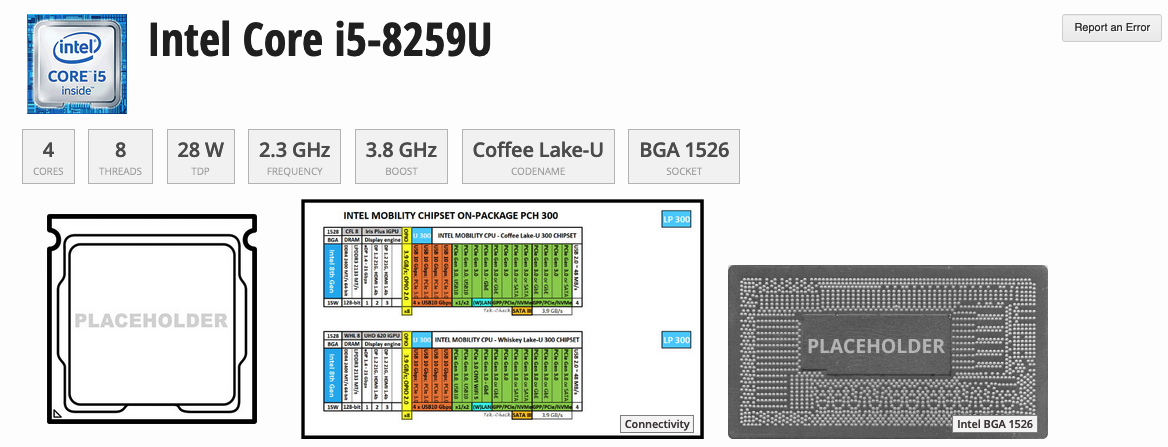
\includegraphics[scale=0.16]{Cisc/2Intel Core i5-8259U.png}}
					\captionof{figure}{Intel Core i5-8259U.}
				\end{minipage}
			}
		\end{tabularx}
	\end{frame}
	
	\begin{frame}{Selezione di un "single-board" pc}
		\begin{center}
			{\Large \textbf{RISC Performance}}
		\end{center}
		\begin{tabularx}{\linewidth}{XX}
			{
				%\vspace*{3cm}
				\begin{minipage}{\linewidth}
					\centering
					\begin{tabular*}{\linewidth}{ l l }
					\multicolumn{2}{c}{\large \textbf{BPI-M6}}\\
					{\textbf{Consumi}}&{15W}\\
					{\textbf{Prestazioni}}&{quad-core(2.1GHz)}\\
					{\textbf{\vspace*{5mm}RAM}}&{\vspace*{5mm}4 GB LPDDR4 }\\
					\end{tabular*}
				\end{minipage}

				\begin{minipage}{\linewidth}
					\centering
					\begin{tabular*}{\linewidth}{ l l }
					\multicolumn{2}{c}{\large \textbf{Odroid-M1S}}\\
					{\textbf{Consumi}}&{10W}\\
					{\textbf{Prestazioni}}&{quad-core(1.8GHz)}\\
					{\textbf{RAM}}&{4 GB LPDDR4 }\\
					\end{tabular*}
				\end{minipage}
			}&{
				\begin{minipage}{\linewidth}
					\centering
					\begin{tabular*}{\linewidth}{ l l }
					\multicolumn{2}{c}{\large \textbf{OPI-5}}\\
					{\textbf{Consumi}}&{20W}\\
					{\textbf{Prestazioni}}&{8-core {\scriptsize (4x Big core 2.4GHz,}}\\
					{}&{\scriptsize 4x Little core 1.8GHz)}\\
					{\textbf{\vspace*{5mm}RAM}}&{\vspace*{5mm}4GB/8GB/16GB LPDDR4 }\\
					\end{tabular*}
				\end{minipage}

				\begin{minipage}{\linewidth}
					\centering
					\begin{tabular*}{\linewidth}{ l l }
					\multicolumn{2}{c}{\large \textbf{RPI-4}}\\
					{\textbf{Consumi}}&{15W}\\
					{\textbf{Prestazioni}}&{quad-core(1.8GHz)}\\
					{\textbf{\vspace*{5mm}RAM}}&{\vspace*{5mm}1GB/2GB/4GB/8GB LPDDR4 }\\
					\end{tabular*}
				\end{minipage}
			}
		\end{tabularx}
	\end{frame}
	
	\begin{frame}{Selezione di un "single-board" pc}
		\begin{center}
			\vspace*{-5mm}
			{\Large \textbf{CISC Performance}}
			\vspace*{2.5cm}
		\end{center}
		\begin{tabularx}{\linewidth}{XX}
			{
				\begin{minipage}{\linewidth}
					\centering
					\begin{tabular*}{\linewidth}{ l l }
						\multicolumn{2}{c}{\large \textbf{Acemagician-T8Plus}}\\
						{\textbf{Consumi}}&{15 W}\\
						{\textbf{Prestazioni}}&{4 Core, 4 Thread 2.3GHz}\\
						{\textbf{\vspace*{5mm}RAM}}&{\vspace*{5mm}16GB DDR4}\\
					\end{tabular*}
				\end{minipage}
			}&{
				\begin{minipage}{\linewidth}
					\centering
					\begin{tabular*}{\linewidth}{ l l }
						\multicolumn{2}{c}{\large \textbf{Acemagician-CK10}}\\
						{\textbf{Consumi}}&{28W}\\
						{\textbf{Prestazioni}}&{4 Core, 8 Thread 2.3GHz}\\
						{\textbf{\vspace*{5mm}RAM}}&{\vspace*{5mm}16GB DDR4}\\
					\end{tabular*}
				\end{minipage}
			}
		\end{tabularx}
	\end{frame}
	
	\begin{frame}{Selezione di un "single-board" pc}
		\begin{center}
			{\Large \textbf{La crisi dei semiconduttori}}
		\end{center}
		\begin{itemize}
			\item La crisi dei semiconduttori è un fenomeno nell'industria dei circuiti integrati che avviene quando la domanda di chip di silicio supera l'offerta.
		\end{itemize}
		\vspace*{3mm}
		\begin{tabularx}{\linewidth}{XX}
			{
				\centering
				\zoombox{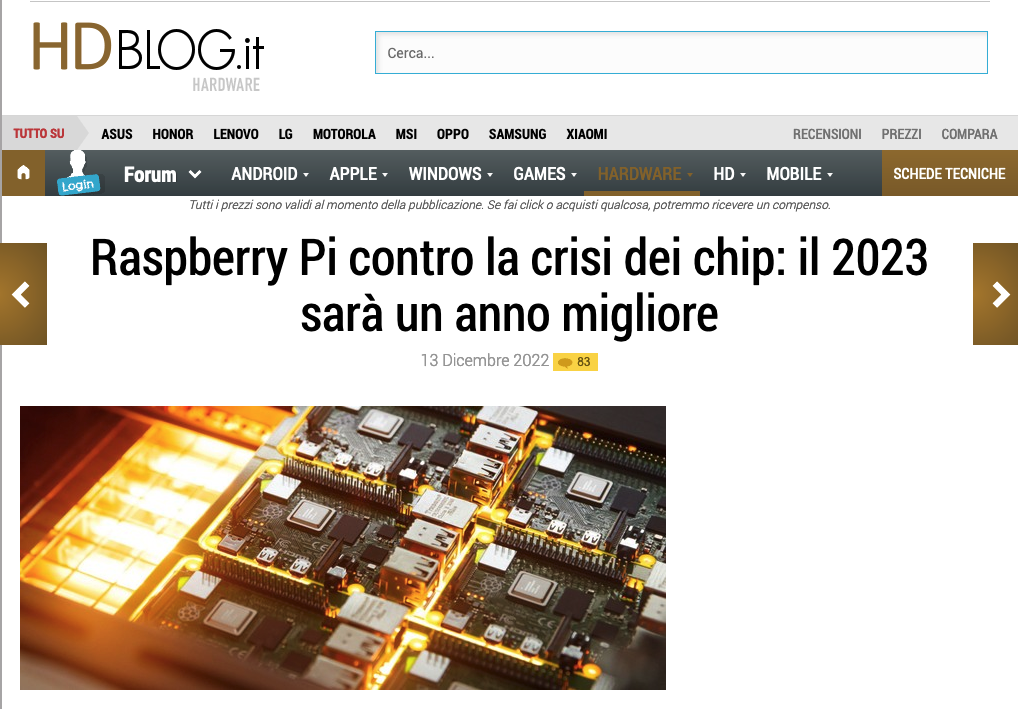
\includegraphics[scale=0.135]{Crisi_semiconduttori/HD_blog.png}}
				\captionof{figure}{\href{https://www.hdblog.it/hardware/articoli/n564270/raspberry-pi-crisi-chip-2023-anno-migliore/}{\textcolor{blue}{Articolo di HDblog.}}}
			}&{
				\centering
				\zoombox{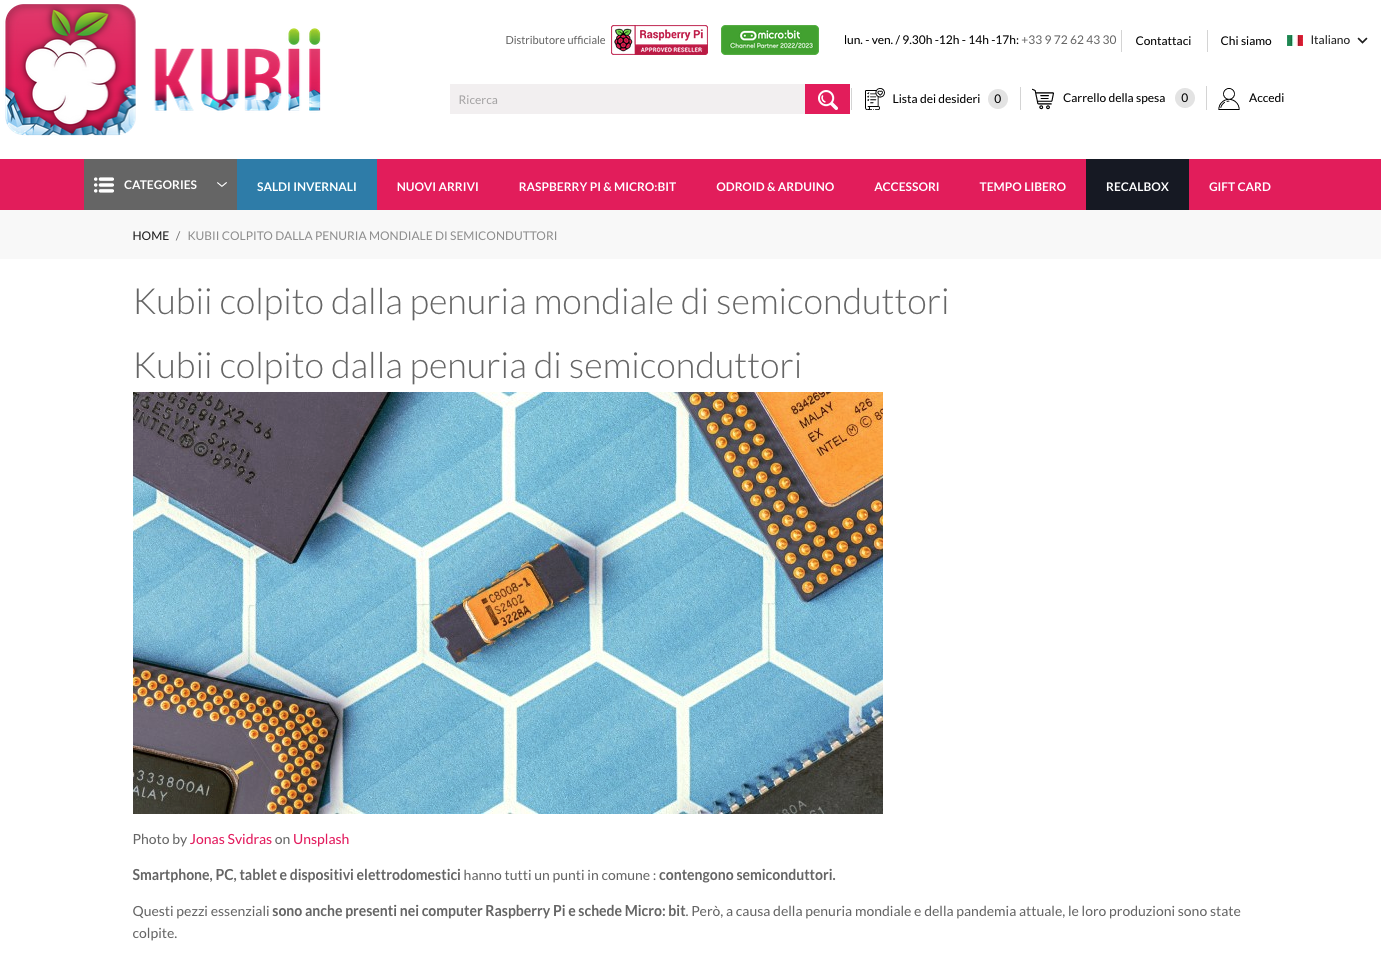
\includegraphics[scale=0.1]{Crisi_semiconduttori/Kubii.png}}
				\captionof{figure}{\href{https://www.kubii.com/it/content/314-Kubii-colpito-dalla-penuria-mondiale-di-semiconduttori}{\textcolor{blue}{Avviso da Kubbii.}}}
			}
		\end{tabularx}
	\end{frame}
	
	\begin{frame}{Selezione di un "single-board" pc}
		\begin{center}
			{\Large \textbf{La scelta finale}}
		\end{center}
		\begin{tabularx}{\linewidth}{XX}
			{
			\centering
			\zoombox{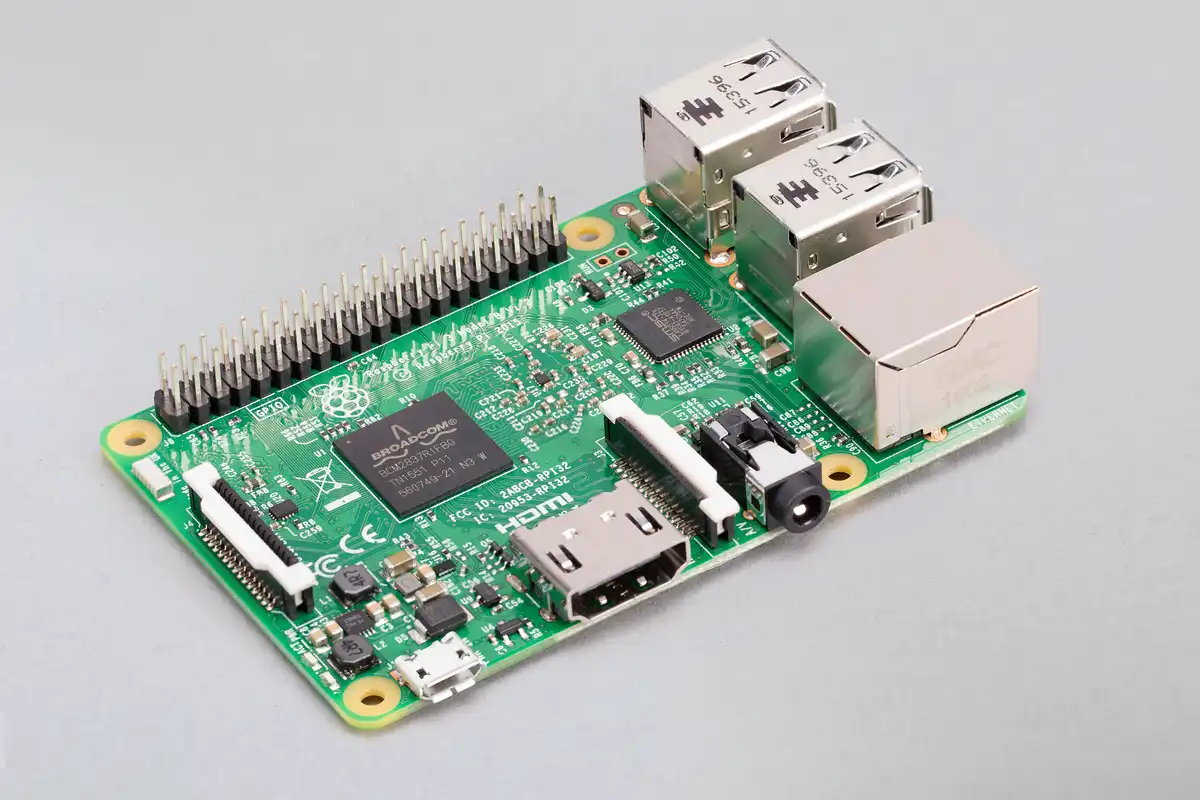
\includegraphics[scale=0.07]{Risc/5Raspberry_pi_3.png}}
			\captionof{figure}{RPI-3.}
			\vspace*{2mm}
			\zoombox{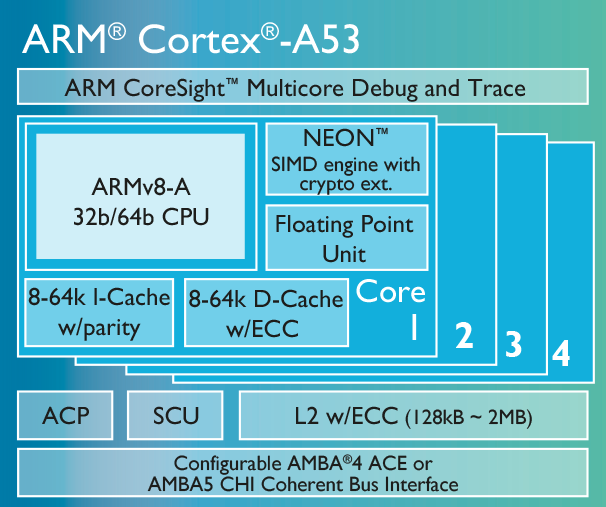
\includegraphics[scale=0.15]{Risc/5BCM-2837.png}}
			\captionof{figure}{BCM-2837.}
			}&{
			\vspace*{0.5cm}
			\centering
			\begin{tabular*}{\linewidth}{ l l }
			{\textbf{Consumi}}&{11W}\\
			{\textbf{Prestazioni}}&{Quad Core 1.2GHz}\\
			{\textbf{RAM}}&{1GB LPDDR2}\\
			\end{tabular*}
			}
		\end{tabularx}
	\end{frame}
	
	\section{La scelta del sistema operativo}
	\begin{frame}{La scelta del sistema operativo}
		contenuto...
	\end{frame}
	
\end{document}